\chapter{Calculation of Condensate Fraction using DMRG Algorithm} \label{chap:CondFrac}
To illustrate the power of the DMRG algorithm, the following numerical analysis was conducted. As the system of interest is the Bose-Hubbard model described in eq. \eqref{BHhamil}, a suitable benchmark for the algorithm is attempting to calculate the critical point of the phase transition between the superfluid and Mott-Insulator. The critical point was determined using the DMRG algorithm in \cite{Kuhner2000} by studying the correlations of the system. Here, an alternative approach is presented, which examines the condensate fraction.\\
According to the Penrose-Onsager criterion, a system is in the superfluid phase if and only if the largest eigenvalue, $\lambda_1$, of the single-particle density matrix, $\rho^{(1)}$, is macroscopic
\begin{equation}
	f_c = \frac{\lambda_1}{N_p} > 0 \; ,
	\label{eq:condensateFraction}
\end{equation} 
where $f_c$ is the condensate fraction, and $N_p$ is the total number of particles \cite{PenroseOnsager}. The condensate fraction can be used to determine which phase dominates the system, as
\begin{align}
	\lim_{N_p \to \infty} f_{c}^{\mathrm{SF}} &\to 1 \label{eq:SF_lim} \\
	\lim_{N_p \to \infty} f_{c}^{\mathrm{MI}} &\to 0 \; , \label{eq:MI_lim}
\end{align}
when the filling-fraction, $n = N_p/L$, is held constant.\\
To calculate the condensate fraction, the ground state of the system was found using a version of the DMRG algorithm implemented in the ITensor library \cite{ITensor}. Using the computed ground state, $\ket{\psi}$, the entries of the density matrix were calculated
\begin{equation}
	\rho_{i,j}^{(1)} = \bra{\psi} \hat{a}_{i}^{\dag} \hat{a}_{j} \ket{\psi} \; .
\end{equation}
Lastly, the condensate fraction was determined through eq. \eqref{eq:condensateFraction}.
The calculation was performed with varying $U/J$ for various system sizes of unit occupancy. The DMRG algorithm was set to perform 5 sweeps with a maximum bond dimension of 200.
In order to gauge the accuracy of the algorithm, the results for system sizes 4-10 were compared to a similar calculation using exact diagonalisation.
\begin{figure}[h!]
    \centering
    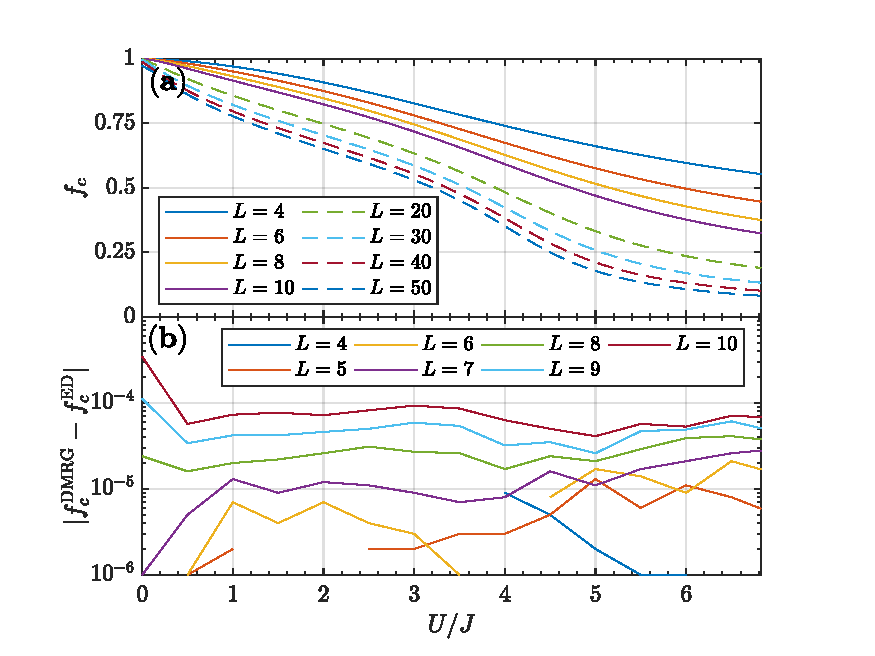
\includegraphics[width=0.7\textwidth]{Figures/CondensateFractionCompare.pdf}
 \caption{\textit{Condensate fraction calculated using the DMRG algorithm with 20 sweeps. The condensate fractions of the smaller systems ($L = 4 \ldots 10$) are compared with result obtained through exact diagonalisation.}}
 \label{fig:CondensateFraction}
\end{figure}
The upper part of figure \ref{fig:CondensateFraction} shows the condensate fraction for various $U/J$ calculated using the DMRG algorithm. In the limit $U/J = 0$, the condensate fraction is unit for the smaller systems, confirming the system is indeed in the superfluid phase. The condensate fraction never reaches zero as $U/J$ increases, since this is only achieved in the thermodynamic limit. However, the condensate fraction does decrease with increasing particle number, as would be expected. The lower half of figure \ref{fig:CondensateFraction}  displays the results of the DMRG calculation compared with exact diagonalisation. For small systems the two approaches obtain very similar results.\\
Attempting to use exact diagonalisation for large systems is futile, due to the exponential scaling of the Hilbert space \cite{Vidal2003}. However, this is not an issue using matrix product states, as the formalism only considers a tiny corner of the Hilbert space by following an area law. 
The dashed lines of figure \ref{fig:CondensateFraction} shows the results of the DMRG calculations for up to 50 particles. The condensate fraction behaves as expected in the $U/J \gg 1$ limit, as it tends towards zero for larger particle numbers. Note, in the superfluid limit the condensate fraction does not quite reach 1, which is due to difficulty of describing long-range correlations when using matrix product states as described in section \ref{sec:sec:CorrelationLength}.
This is not an issue for smaller systems, as the correlation length is limited by the system size. \\
Some measures can be taken to minimize errors, when using the DMRG algorithm. Accurately describing long range correlations requires multiple sweeps, as the algorithm has to iteratively approximate an almost constant function with a series of exponentials. Figure \ref{fig:sweepdependence} displays the condensate fraction in the Superfluid limit as a function of number of sweeps. Clearly, performing more sweeps yields a better result.
\begin{figure}[h!]
    \centering
    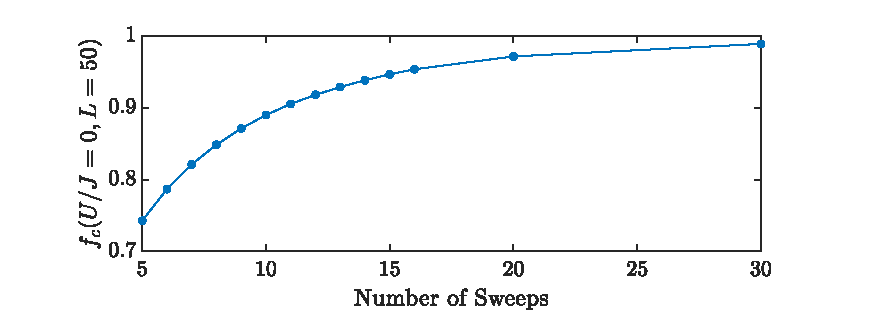
\includegraphics[width=0.7\textwidth]{Figures/CFsweeps.pdf}
    \caption{\textit{Condensate fraction as a function of number of sweeps of the DMRG algorithm in the superfluid limit. A max bond dimension of $D = 250$ was used.}}
    \label{fig:sweepdependence}
\end{figure}
Furthermore, increasing the maximal bond dimension, $D$, results in a more accurate long-range representation of correlations. Thus, calculating correlation functions for various values of $D$ is a great way of estimating the convergence of the correlations for a given length scale \cite{schollwock}.\\

In \cite{Kuhner2000} the critical point of phase transition between the Superfluid and Mott-Insulator is determined as $\left( \frac{U}{J} \right)_{crit} = 3.37$. The result is achieved through examining the correlations of the systems. While correlations in Mott-Insulators decay exponentially, superfluids have a decay of correlations following the power-law given in eq. \eqref{sec:correlationFunctions}. The interface between the two phases has correlations following a power law determined by the Luttinger liquid parameter. The critical point, which is located at the tip of the Mott-lobes, is computed by determining the point at which the Luttinger liquid parameter is $K =  \frac{1}{2}$ \cite{Kuhner2000}.\\
Examining figure \ref{fig:CondensateFraction}, one notices a hump on the graph in the vicinity of the critical ratio, but no clear indication of a phase transition is present. In the thermodynamic limit one would expect the condensate fraction to drop to zero as the critical ratio is reached (as observed in 2D by \cite{Spielman2008}). However, at 50 particles the condensate fraction is only around $ f_c = 0.5$. One could extrapolate data from computations using different particle numbers in order to determine the location of the critical point. However, this would require computations using larger systems in order to minimize the boundary effects.